\chapter{Regulatory Licensing Obligations}
\section{Eligibility for Licensing}
The licensing requirements are multifaceted, covering operating systems, client access, management suites, and cloud services.

\begin{figure}
    \centering
    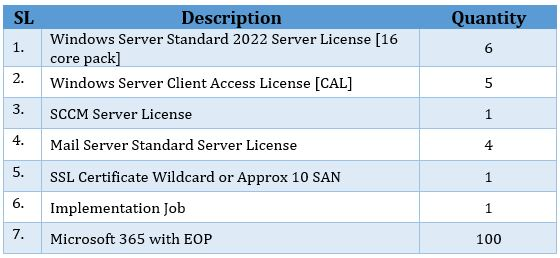
\includegraphics[width=0.5\linewidth]{Chap8/BOM.JPG}
    \caption{Licensing Requirement.}
    \label{fig:placeholder}
\end{figure}

Windows Server 2022 License:
The requirement for six "Windows Server Standard 2022 Server License [16 core pack]" units indicates a substantial virtualized environment. Windows Server licensing is core-based, not per server. Each physical server must be licensed with enough core licenses to cover all its physical cores, with a minimum of 16 cores per server. Each "16 core pack" covers 16 physical cores. To determine the number of physical servers, we must understand that the Standard edition permits two Virtual Machines (VMs) per fully licensed host. Therefore, six licenses could represent three physical servers, each fully licensed with enough core packs for their CPU cores, granting the right to run a total of six Windows Server VMs.

Client Access Licenses (CALs):
The purchase of only five "Windows Server Client Access License [CALs]" is a critical point of analysis. CALs are required for every user or device that accesses the Windows Server's services (like file sharing, or user authentication). With only five CALs, this infrastructure is severely restricted in the number of users who can legally access it. This implies the servers are intended for backend infrastructure or application-hosting roles that are not directly accessed by a large number of users, perhaps only by administrators. This must be carefully planned to avoid compliance issues.

System Center Configuration Manager (SCCM) License:
"SCCM Server License" is required to manage this environment. SCCM is a powerful tool for managing PCs, servers, and mobile devices. The single license covers the management server itself. However, to manage the clients (the 100 Microsoft 365 users and the servers), separate SCCM Client Management Licenses (CMLs) are required for each device being managed.

Mail Server Licensing:
Four "Mail Server Standard Server License" units suggest a dedicated, on-premises Exchange Server. Similar to Windows Server, this is likely licensed per core of the physical host(s) where the mail server VMs will run. The quantity of four licenses points towards a need for running multiple mail server VMs, possibly for high availability, dedicated roles (e.g., front-end transport, mailbox server), or to handle the load for the 100 Microsoft 365 users in a hybrid configuration is used.

SSL Certificate:
The "SSL Certificate Wildcard or Approx 10 SAN" is not a traditional software license but a critical security and trust requirement. A wildcard certificate secures a main domain and all its subdomains (e.g., *.company.com). A SAN (Subject Alternative Name) certificate can secure up to 10 distinct fully qualified domain names. This certificate will be essential for securing web services, the mail server, the SCCM management point, and other internal or external sites, ensuring encrypted communication.

Implementation Services:
The "Implementation Job" is a professional service, not a software license. However, its inclusion is vital. It covers the labor for the complex task of installing, configuring, and integrating all the licensed products according to their specific requirements and best practices. This ensures the entire licensed ecosystem is deployed correctly and efficiently.

Microsoft 365 with EOP:
The 100 "Microsoft 365 with EOP" licenses represent a shift to a cloud-based productivity and collaboration suite. This is a subscription-based User Subscription License (USL). Each of the 100 users will have the right to use the included applications (like Office apps) and services. EOP (Exchange Online Protection) provides cloud-based email filtering for security. It is important to note that this subscription may include cloud-based services that overlap with on-premises licenses (like the Mail Server), suggesting a potential hybrid environment or a planned migration.

Compliance:
The licensing requirements for this project are a hybrid of perpetual/core-based licenses (Windows Server, SCCM), subscription/user-based licenses (Microsoft 365), and client-access licenses (CALs). A significant consideration is the potential overlap and dependency between products. For instance, the on-premises servers and the 100 cloud users must be correctly synchronized, likely via Azure AD. Furthermore, the stark contrast between the small number of CALs and the large number of Microsoft 365 users needs a clear architectural justification to maintain licensing compliance. Proper documentation and understanding of the Microsoft Product Terms are essential to ensure this entire ecosystem is both functional and legally licensed.

Active Directory Foundation: Windows Server licenses with sufficient
Client Access Licenses (CALs) for all users and devices are mandatory for domain
controllers. Exchange Server Licensing: An Exchange Server license is required, typically Standard Edition for most hybrids, along with Exchange Server CALs for each
user. Core Office 365 License: User Subscriptions Licensing (USL) for Microsoft 365
or Office 365 E3/E5 is the primary requirement for cloud mailboxes and services.
Hybrid Feature Key: The free, Microsoft-supplied Hybrid Edition license enables advanced hybrid features without needing a full, paid Exchange Server license. Azure
AD Connect: This crucial synchronization tool is included with the Office 365 subscription at no additional cost. Identity Foundation: Azure AD is included, but a
premium Azure AD P1 license is often recommended for enhanced hybrid identity
security. Management Overhead: Licensing covers the on-premises Exchange server
used solely for management tasks in a "minimal hybrid" configuration. Client Access
Licensing: Ensure Microsoft 365 plans include the rights for desktop Office apps or
purchase them separately for users.



